\subsubsection{11.02.15 (Competition)}
\begin{center}
	1-st day of competition "Robofest-2015"
\end{center}
Today there was technical day. We trained debugged autonomous period and communicated with another teams.\newline

Firstly we talked with all FTC teams. There were 33 teams.We learned about opportunities and strategy of every team. We got a dates about all robots. Also we gave to all teams the lists with short information about our strategy and opportunities. So we drew attention to our team and we has more chances that another team will choose us for the final matches.\newline

In addition we gave our engineering book to the judges.\newline

Improvements that were done:
\begin{enumerate}
	\item It was found that the right corner of the bucket hooks the wire that connect servo that overturns bucket with servocontroller. So the corner was cut and it was glued the patch. The bucket stopped hook the wire.
	\begin{figure}[H]
		\begin{minipage}[h]{0.47\linewidth}
			\center{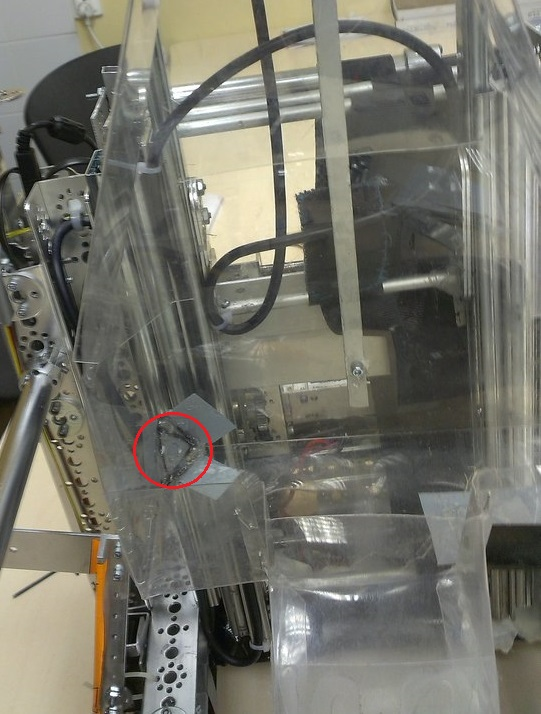
\includegraphics[scale=0.25]{days/11.02.15/images/01}}
			\caption{The cut corner}
		\end{minipage}
		\hfill
		\begin{minipage}[h]{0.47\linewidth}
			\center{
\includegraphics[scale=0.7]{days/11.02.15/images/02}}
			\caption{Larger image}
		\end{minipage}
	\end{figure}
	
	\item We decided to concentrate on the programme of autonomous period from the parking zone because the most part of teams did autonomous period from the ramp better than from the parking zone.
	
		\item The guideway for balls was fixed only on the slats. So it staggered. To prevent this it was decided to install the stopper that that limits backlash of the guiedeway. So the problem was fixed.
	\begin{figure}[H]
		\begin{minipage}[h]{0.2\linewidth}
			\center  
		\end{minipage}
		\begin{minipage}[h]{0.6\linewidth}
			\center{
\includegraphics[scale=0.2]{days/11.02.15/images/03}}
			\caption{Stopper}
		\end{minipage}
	\end{figure}
	
\end{enumerate}
\fillpage
